\chapter{Introduction}
\thispagestyle{empty}
\label{chap:introduction}
A blank piece of paper is God's way of telling us how hard it to be God\\
- Sidney Sheldon (1917 - 2007)\\\\

\emph{This first chapter is to introduce the reader to concepts such as gene, chromosome 
and DNA all the way up to Multiple QTL mapping (MQM) and Genome Wide Association Studies 
(GWAS). This chapter provides the necessary background information for the following 
chapters. Its is however only a short historical overview of systems genetics, and 
introduces only concepts and software used in the analysis of heritable phenotypes that 
are relevant to this thesis. }

\null
\vfill
\newpage

\section{Introduction}
Systems genetics is the interdisciplinary field which deals with the effects of perturbation 
and natural variation measured at a all possible levels of a biological system. It takes a 
more holistic approach to understanding biological systems. In the last 20 years our ability 
to take large scale measurements from the transcriptome, metabolome and proteome have 
improved dramatically leading to a virtual avalanche of biological data.

Phenotype variation / diversity observed is the consequence of a mixture of variation 
originating at the DNA level (DNA), the environment (Env), and an error component (Err).

$$ Phenotype = Env + DNA + DNA * Env + Err $$

Partitioning of observed variation into this formula is of critical importance 
to understanding the contribution of genetics and environment to the biological 
processes observed. Understanding how a system works and reacts to different 
environments, allows modification of the system to better suit our needs or 
environmental requirements. Knowledge about DNA variation allows to optimize 
breeding of animals and plants, explore the genetic basis of human diseases, 
improved production of chemicals, and so forth.

Variation observed at the DNA level can be measured using genotyping (AFLP, RFLP, 
SNPs, Sequencing) techniques, allowing to create detailed maps of DNA inheritance 
within a population and track the origin of DNA through many generation.

At the phenotype end of the spectrum new high throughput technologies have also 
been developed to mass produce phenotypes measurements using automated phenotyping. 
Automated phenotyping allow thousands of simultaneous measurements at all the 
different endophenotype levels such as: metabolome, proteome, transcriptome. These 
new technologies such as tiling arrays, RNAseq, High throughput proteomics and 
metabolomics now enable us to measure all levels from the DNA to the observed 
phenotype at minimal costs.

How the activity of DNA is regulated by signals from all molecular levels and modified by 
signals from the environment is the focus of systems genetics. The use of computational 
tools in understanding how genetics and environment intertwine is the central in the 
field of systems genetics to deal with the large amounts of phenotype and genotype data.

Variation observed at levels 'further away' from the genome such as: transcriptome, 
proteome, metabolome, all the way up to classical phenotypes form a complex interplay 
between DNA and environment. This interplay has proven to be challenging to unravel.The 
following chapters of this thesis will go into our solutions to these issues, 
infrastructure created, methodologies developed, and their application in current 
research. First some (historical) background to provide a solid foundation  and outline
the context of the following chapters.

\section{History (1800-1930)}

The field of genetics is a relatively old field, and is founded when Gregor 
Mendel publishes his work on the inheritance of phenotypes in pea plants. 
His work described in 'Versuche \"uber Pflanzen-Hybriden' in 1865-1866 
\cite{Mendel:1866} gives us Mendel's Laws of Inheritance. He observed that 
crossing two plants with different colors of flowers leads to an offspring 
population with predictable color ratios. He postulated the idea of heredity 
units and stated that each individual carries two of these resulting in a 
single phenotype. Each heritable units is received from one of the parents, 
but which one of the two units from the parents gets passed to a child is random 
(Law 1 - Segregation).

These two units are not equal, a dominant unit (color 1) overruled another 
unit (color 2 - recessive). Mendel studied more phenotypes in his pea plants 
besides color. Now it is known that Mendel was fortunate to select 
phenotypes which are caused by a single genes and are inherited independently. 
Mendel also observed this when comparing inheritance of multiple phenotypes. 
He concluded that a unit of inheritance is passed from parent to child in an 
independent fashion compared to other units of inheritance 
(Law 2 - Independent Assortment).

Mendel's work was not fully recognized until 30 years later, when his work was 
rediscovered by Hugo de Vries, Carl Correns en Erich von Tschermak who (re) defined the 
rules for Mendelian Genetics \cite{deVries:1889} providing biologist for the first 
time with a mathematical framework to study heritability of phenotypes caused by a 
single genetic unit.

Twenty years after the rediscovery of Mendel's Laws in 1913, careful observations of 
Thomas Hunt Morgan introduced an addition to Mendel's theoretical work. He observed 
that some phenotypes in his \emph{Drosophila melanogaster} mutant flies are inherited 
together, in conflict with Mendel's Laws (which state independent inheritance of 
genetic units). He calls this phenomenon genetic linkage. This concept is also commonly 
explained as beads on a string: in which multiple genetic units linked together. Two beads 
close together are tightly linked are and almost always inherited together. While 
two beads far apart are less linked and can be separated by meiosis. Different 
strands are independently inherited allowing for Mendelian inheritance by two beads 
on two different strings.

Sturtevant a student of Morgan used his mentors linkage theory between phenotypes 
as a distance measurement between units of inheritance. He created the first genetic 
map of \emph{Drosophila melanogaster} 40 years before the discovery of the DNA molecule, 
while molecular mechanisms were still unknown. Sturtevant genetic map, based on 
phenotypes, allowed genetics based on careful observation of segregating phenotypes in 
large populations of flies, and then determining their distance relative to other 
phenotypes.

\section{DNA and QTLs (1930-1990)}

The discovery of DNA as the carrier of heritability in 1944 by Avery, MacLeod and McCarty 
\cite{Avery:1944} and the discovery of its structure by Watson and Crick.in 1953 
\cite{Watson:1953} was the long sought after molecular basis for genetics. After the 
discovery of restriction enzymes by Luria and Human \cite{Luria:1952} it was possible 
to cut DNA and investigate the different (lengths of) fragments produced.

In the end of the 1980s everything was there for the next big step in genetics. Three 
papers were published which detail the use of RFLP linkage maps to localize genes 
responsible for variation in quantitative phenotypes. These three papers by David Botstein 
and Eric Lander \cite{Lander:1986, Lander:1987, Lander:1989} form the basis for modern 
day linkage analysis and genome wide association studies. 

\begin{figure}[h!]
 \centering
    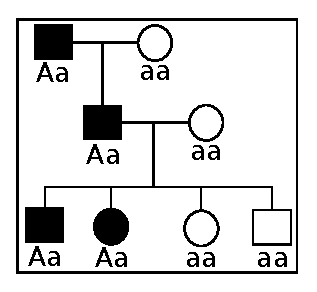
\includegraphics[width=0.4\textwidth]{eps/image_1_2}
  \caption[Example of pedigree based linkage analysis.]
    {Example of a hypothetical pedigree on which linkage analysis can be performed. Here we show a 
    hypothetical pedigree of individuals within a family (2 generations), squares represent 
    male individuals while circle are females. The phenotype is shown encoded by the fill 
    color of the shape (Black = affected, White = not affected).  In this example pedigree, 
    the "A" allele segregates with the disease. It is shared identical-by-descent in all 
    affected individuals. }
    \label{fig:pedigree}
\end{figure}

In linkage analysis, DNA is tracked from parents to children. This allows to build so called 
genetic familie trees or pedigrees (See fig. \ref{fig:pedigree}) in which segregation of a phenotype (or 
disease) is displayed. If we find a genetic region which co-segregates with the disease we can assume this DNA and 
disease are linked, and asses the strength of the linkage observed. By using experimental 
crosses derived from inbred parents the need to build up complex pedigrees is avoided, while 
retaining the advantage of being able to trace back the DNA to the founder strains. Also inbred 
populations provide high statistical power at the cost of reduced resolution for QTL mapping. 
This reduction in resolution is caused by the lack of recombinations in populations which are 
generally small (20 to 1000 individuals).

Association analysis is done in outbred populations, where tracking of the origin of the 
DNA is hard or impossible. However molecular markers still allows to get information 
about the underlying DNA. We can use e.g. Single Nucleotide Polymorphisms (SNPs) and associate 
a phenotype with this genetic marker. The advantage of this approach is that resolution is 
very good, because we have a high number of recombinations in outbred populations. However 
because of this large quantity of markers statistical power to detect effects are limited.

Heritable phenotypes could be mapped to genomic locations using a combination of DNA 
restriction enzymes, Mendel's inheritance laws and Hunt's linkage theory. Together these 
methodologies and theories provide the experimental and statistical background to 
analyse heritability in any population. Linkage and Association analysis are still the 
foundation of population genetics research today. More sophisticated tools and algorithms have been 
developed and are used, but the basic theory remains the same. Some of these more 
advanced methods are discussed in the next section to sketch a background for the work 
presented in this thesis.

\begin{figure}[h!]
 \centering
    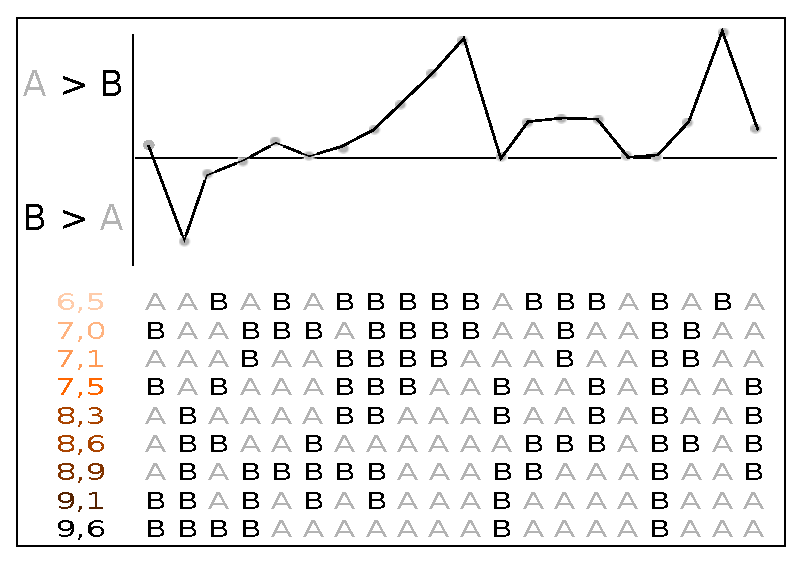
\includegraphics[width=0.4\textwidth]{eps/image_1_1}
  \caption[Effect scan across the genome.]
    {Example of how an effect scan is done using a single phenotype and a matrix of genotypes (A or B).}
    \label{fig:effectscan}
\end{figure}

\section{From Phenotypes to Genetical Omics and GWAS (1990-2010)}

Observed phenotype expression is often more complex than a single causative gene. 
To model these more complex interactions extension of the basic model for QTL mapping is 
necessary. Extending the model can be done by incorporating sources of variation. This allows 
us to associate / partition the observed variance to either environmental factors (E) or a 
genetic loci (G).

To include G components into the model Multiple QTL Mapping (MQM) can be used. MQM belongs 
to a family of QTL mapping methods, that include Haley-Knott regression \cite{Haley:1992} 
and composite interval mapping CIM \cite{Zeng:1994}. MQM combines the strengths of 
generalized linear model regression with those of interval mapping \cite{Jansen:1993, Jansen:1994b}. 

\begin{table}[h]
  \centering
  {\footnotesize
  \begin{tabular}{ | c | l | l | }
    \hline
    {\bf Molecular level} & {\bf Molecule} & {\bf Technology}\\
    \hline
    \hline
\rowcolor{gray!35}    Genome          & DNA                & RFLP \cite{Lander:1986} \\
\rowcolor{gray!35}    Genome          & DNA                & SNP chips \cite{Hacia:1999} \\
\rowcolor{gray!35}    Genome          & DNA                & DNA sequencing \cite{Mardis:2008} \\
    \hline
    EpiGenome       & DNA methylation    & Bisulfite sequencing \cite{Hayatsu:2007} \\
    EpiGenome       & DNA methylation    & ChIP-on-chip \cite{Collas:2010} \\
    EpiGenome       & DNA methylation    & ChIP-Seq \cite{Park:2009} \\
    \hline
    \hline
\rowcolor{gray!35}    Transcriptome   & RNA          & Microarray \cite{Lashkari:1997}, Tiling array \cite{Lee:2013} \\
\rowcolor{gray!35}    Transcriptome   & RNA          & RNA-Seq \cite{Wang:2009}\\
    \hline
    Proteome        & Proteins     & 2D gel electrophoresis \cite{O'Farrell:1975}\\
    Proteome        & Proteins     & Mass Spectometry \cite{Deshaies:2001}\\
    Proteome        & Proteins     & Antibody protein chip \cite{Fasolo:2009} \\
    \hline
\rowcolor{gray!35}    Metabolome      & Metabolites  & Mass Spectometry \cite{Aebersold:2003} \\
\rowcolor{gray!35}    Metabolome      & Metabolites  & Nuclear magnetic resonance \cite{Espina:2009} \\
    \hline
  \end{tabular}
  }
  \caption[Overview]{Overview of current technologies}
\end{table}

Genetical Genomics is the concept that views endophenotypes (RNA, Protein and Metabolite abundance) 
as common phenotypes wich can be mapped in bulk to the genome similar to classical 
phenotypes \cite{Jansen:2001a}. Using natural occurring variation and new omics tools allows us 
to track variation from the genotype all the way up to the classical phenotypes. Allowing 
genetics to go from individual QTLs to a system wide approach of analyzing QTLs at all known 
molecular levels called Systems Genetics \cite{Threadgill:2006}. Studies in model organisms 
have shown high heritability's for endophenotypes such as gene expression making these phenotypes 
ideal targets for QTL mapping \cite{Brem:2002}. 

In 2003 R/qtl was developed to provide reference implementations for QTL mapping. R/qtl is 
an extensible, interactive environment to map quantitative trait loci (QTL) in experimental c
rosses. It is implemented as an add-on package for the freely available and widely used 
statistical language/software R \cite{R:2009}. The main focus of R/qtl is to provide 
the mouse community with different QTL mapping methodologies, and allow to deal with the 
the aberrant segregation X chromosome. Furthermore it supports different types of inbred 
populations such as BackCross, F2, Recombinant inbred lines and 4-way RILs. \cite{Broman:2003}

When mapping gene expression or protein abundance current knowledge of protein and DNA sequence 
allows us to locate their template on the genome. When QTL mapping resolution allows we can even 
distinguish between traits mapping in the proximity of their respective gene (\emph{cis}-eQTL) 
or to other regions in the genome (\emph{trans}-eQTL). This information can be summarized into 
so called cis-trans plots, where the X-axis is the location of the eQTL and the Y-axis the genetic 
location of the trait. Often so called trans-bands are observed, hotspots of many \emph{trans}-
eQTL mapping to a common region in the genome \cite{Breitling:2008a}, which are used to infer 
biological meaning and reconstruction co-expression and/or co-regulatory networks.

In the last decade Genome Wide Association Study (GWAS) have identified thousands of genetic 
variants that are associated with human disease\cite{Hindorff:2009}. For reliable results GWAS 
needs a large cohort of genotyped and phenotyped individuals. Large consortia are working 
together to gather large amounts of human expression data from many different tissues. This 
data is then used in meta analysis leading to eQTL GWA studies with even larger sizes 
(5000+ individuals) \cite{Lude:2011}, leading to more reliable results and enabling discovery 
of new modifiers of human gene expression.

It is known that many factors, such as effects on intermediate molecular phenotypes, influence 
the relationship between genotype and the eventual development of disease. It has also been 
observation that many of the disease-predisposing variant are noncoding, suggests a regulatory 
function for these variants. And it has been shown that many disease-predisposing variants 
(e.g. single nucleotide polymorphisms (SNPs)) affect the expression of nearby genes (i.e. 
\emph{cis}-eQTLs)\cite{Powell:2012, Lude:2011, Zeller:2010}

\begin{figure}[h!]
 \centering
    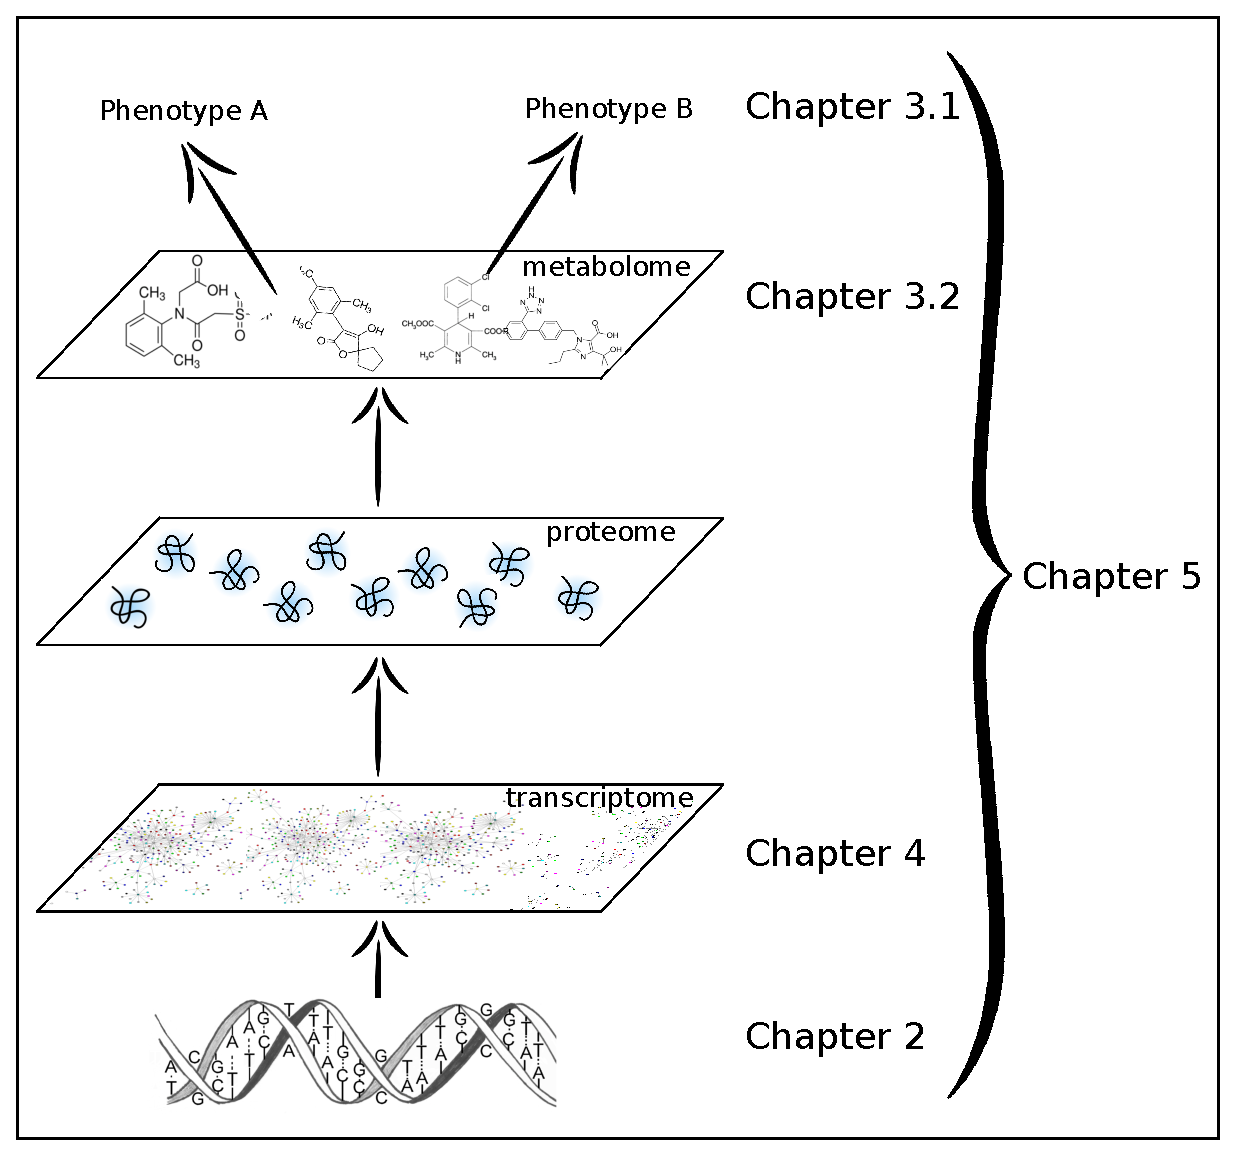
\includegraphics[width=0.6\textwidth]{eps/image_1_3}
  \caption[ThesisLayout.]
    {Schematic figure showing to which molecular level each chapter is related. Molecular 
    level here depicted are drawn from genome (bottom) to phenome (top), arrows indicate 
    how genetic information is transfered from level to the level as by the current by 
    the biological 'dogma'.}
    \label{fig:layout}
\end{figure}

\section{Thesis contributions (2010-2014)}
Chapter \ref{chap:pheno2geno} details how Pheno2Geno is developed for high-throughput 
generation of genetic markers and maps from molecular phenotypes. Pheno2Geno selects 
suitable phenotypes that show clear differential expression in the founders. Pheno2Geno 
uses mixture modeling to select phenotypes showing segregation ratios close to the 
expected mendelian segregation ratios and transform them into genetic markers suitable 
for map construction and/or saturation. Pheno2Geno analyses the candidate genetic 
markers and excludes those showing multiple QTL, epistatically interacting QTL, and QTL 
by environment interactions to provide a set of robust markers for QTL mapping protecting 
against genetic markers from a non genetic origin.

Chapter \ref{chap:mqm} highlights the integration of the Multiple QTL mapping algorithm 
into R/qtl. In sections (\ref{chap:mqm}.1 and  \ref{chap:mqm}.2) we show the performance 
of MQM on experimental data from a cross of \emph{A. thaliana} Bayreuth x Shahdara. We 
focus on the developing seeds in this cross and try to find genetic factors underlying 
changes we observed in the phenome and metabolome.

Chapter \ref{chap:ctlmapping} -  Shows our current work on understanding differences in 
correlation observed when mapping two traits onto the genome. We show that there is a high 
overlap between CTL mapping and using an G:E interaction model, and use this interaction 
model in data form a human genome wide association study (GWAS) to detect cell type specific 
eQTL in whole blood. We show that low effect QTLs observed in samples can be explained by 
compensating for the relative number of neutrophils observed, or predicted. Improving our 
power to detect QTLs and enabling us to assign cell type labels to observed \emph{cis}-eQTL 
effects.

Chapter \ref{chap:xqtlwormbench} - Details our work to provide infrastructure for the Life 
Sciences. We advocate the use of Generators to create software and propose a datamodel (XGAP) 
to store phenotype and genotype data. Combining these two approaches we developed: xQTL 
workbench a scalable web platform for the mapping of quantitative trait loci (QTLs) at 
multiple levels such as gene expression (eQTL), protein abundance (pQTL), metabolite 
abundance (mQTL) and phenotype (phQTL) data. Popular QTL mapping methods for model organism 
and human populations are accessible via the web user interface. Large calculations scale 
easily on to multi-core computers, clusters and cloud computing.
